\subsection{Introducción}

	En el trabajo que realizaron Wang et al., los autores identificador el problema que había al detectar y reconocer palabras en imágenes naturales. Ellos identifican, que si bien las actuales aplicaciones de OCR se manejan bien con documentos escaneados, todavía encuentran problemas cuando tratan de procesar texto adquirido en entornos naturales (también referido como texto de escena). Este tipo de texto se ha vuelto más frecuente debido al aumento de dispositivos que son capaces de extraer dicha información, sean estos celulares, tabletas o cámaras.
	
	Con la salida del primer dataset público denominado \textit{ICDAR} en 2003, los autores del mismo lo establecieron como punto común de referencia. Esto fue con el objetivo de ver cual era el estado del arte de los algoritmos de reconocimiento de texto en imágenes naturales. Observaron que habían imágenes con texto que los motores de OCR del momento no podían procesar, por lo tanto, decidieron dividir el problema general que era reconocer palabras en escenas naturales en tres subproblemas:
	
	\begin{itemize}
		\item La clasificación de caracteres recortados (ver Figura \ref{fig: Caracteres recortados}).
		
		El reconocimiento de caracteres recortados de escenas naturales es un desafio que requiere tener presente algunas cosas. Inicialmente, y como se mostrará más adelante, existe el problema de que algunos caracteres no son fácilmente diferenciables de su versión mayúscula (para los caracteres alfabéticos). Incluso, es posible confundir algunos de ellos con caracteres numérico u otros símbolos. Esto resulta de la falta de ``contexto'' en que se encuentra cada caracter, es decir, no poder tener las imágenes originales de donde fueron extraidas para poder comparar. Es común que surgan este tipo de problemas al momento de clasificar.
				
		Otro elemento que se tiene que tener presente al momento de clasificar caracteres, es el tipo de características locales que se van a obtener de cada imagen. Como se ha explicado en la sección \ref{subsection:feature}, las características son importantes dado que representa los aspectos o cualidades más significativas de un objeto. Si se hace una buena elección de las características locales, se va a ver reflejado en la performance de clasificación.
		
		Las condiciones en que fueron tomadas las imágenes donde se extrajeron los caracteres influye posteriormente en su reconocimiento. Se puede realizar un pre-procesamiento que ayude a ``limpiar'' la imagen para poder facilitar su reconocimiento posterior.
		
		\item Detección de zonas con texto en la imagen completa (ver Figura \ref{fig: Zona texto}).
		
		Para poder resolver este problema, se debe considerar que las palabras que conforman el texto a detectar, pueden estar a diferentes escalas. Tal es el caso del texto de casi la mayoría de los carteles publicitarios que es posible encontrar en las calles de una ciudad. Otro factor a considerar es la inclinación del texto, pués este puede encontrarse inclinado en cualquier ángulo. Además, esta tarea se dificulta si consideramos, al igual que en el reconocimiento de caracteres, las condiciones de la imagen (iluminación, distorsiones, estilo y fuente de las palabras en el texto, etc).
		
		En el trabajo de Chen H. et. al. \cite{ChenH11}, los autores destacan que hay dos categorías al momento de diferenciar las técnicas de reconocimiento de texto. La primera categoría, son las técnicas \textit{basadas en textura} (\textit{texture based} de su traducción al inglés) que destacan al texto como una ``textura'' especial que es distinguible del fondo. Las características se extraen de ciertas regiones de la imagen y se utiliza un clasificador para identificar la existencia de texto. La segunda categoría, son las técnicas basadas en \textit{componentes conectados} (\textit{connected component} de su traducción al inglés), donde se extraen regiones de la imagen y se utilizan restricciones geométricas para descartar candidatos que no sean texto.
		
		%Las soluciones a este problema varian desde combinar varios algoritmos en un pipeline multi-etapa \cite{•}\cite{•} a clasificadores entrenados con características editadas a mano. En cuanto a las características se incluyen los descriptores de texturas, los bordes y los contextos de formas. 
		
		\item El reconocimiento de palabras recortadas (ver Figura \ref{fig: Reconocimiento palabras}).

		El proceso para poder reconocer palabras recortadas depende de poder reconocer los caracteres que conforman estas palabras. Suponiendo que la etapa de reconocimiento de caracteres es buena, la pregunta es cómo detectar la palabra en base a los caracteres clasificados anteriormente. Una solución la proporciona Wang Y Belongie en \cite{WB10} donde, en base a un lexicón (conjunto de palabras), miden la configuración de cada caracter de cada palabra en la imagen. Los autores representan una palabra usando \textit{estructuras pictóricas} (\textit{pictorial structures}, de su traducción al inglés). Una estructúra pictórica es un modelo que considera el costo de emparejar partes individuales (cada carácter) con ubicaciones en la imagen. Básicamente toma la ubicación y el puntaje de los caracteres detectados como entrada y encuentra la configuración óptima para una palabra en particular \cite{wang}.	
		
		El uso de un lexicón para el reconocimiento de palabras es una técnica común \cite{WWI1959}\cite{CPPJ05}. Sin embargo, su uso tiene algunas desventajas. En palabras de Weinman et. al. \cite{JEA}, uno de los mayores inconvenientes de los lexicones es el tiempo que se tarda en examinar palabras candidatas en un lexicón grande.
		
	\end{itemize}
	
	\begin{figure}[htbp]
		\centering
  		\centerline{ 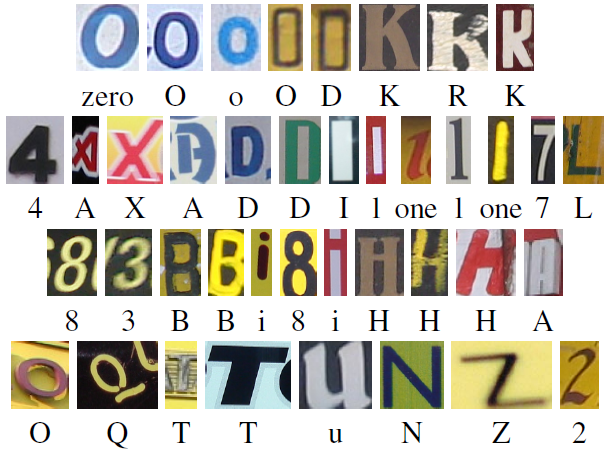
\includegraphics[scale=0.5]{img/hog/confusing_english.png} }
		\caption[Clasificación de caracteres recortados]{Conjunto de caracteres recortados. Imagen extraida del paper de T. E. de Campos et. al. \cite{dCBV09}}
		\label{fig: Caracteres recortados}
	\end{figure}
	
	\begin{figure}[htbp]
		\centering
		\centerline{ 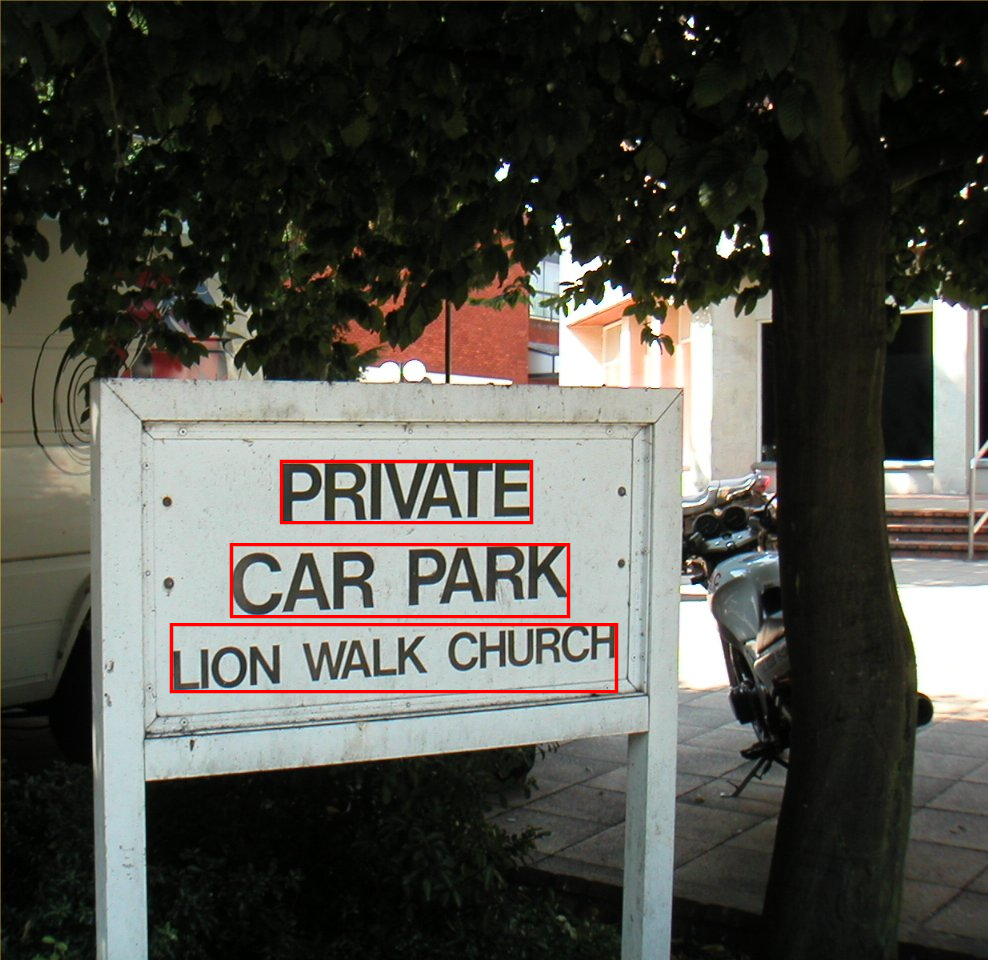
\includegraphics[scale=0.25]{img/zone_with_text.png} }
		\caption[Detección de zonas con texto]{Imagen natural donde las zonas con texto están encasilladas.Imagen tomada del sitio \url{http://libccv.org/post/introducing-ccv-milestone/} }
		\label{fig: Zona texto}
	\end{figure}
	
	\begin{figure}[htbp]
		\centering
		\centerline{ 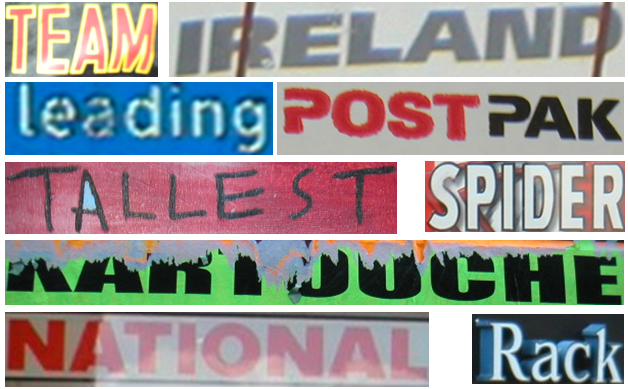
\includegraphics[scale=0.5]{img/cropped_words.png} }
		\caption[Reconocimiento de palabras recortadas]{Conjunto de palabras recortadas de diferentes escenas naturales. Imagen extraida del sitio de \textit{Graphics and Media Lab}, \url{http://graphics.cs.msu.ru/en/science/research/machinelearning/text}}
		\label{fig: Reconocimiento palabras}
	\end{figure}

	Dada esta problemática, Wang et al. se enfocaron en un caso especial del reconocimiento de texto de escena donde tenían a disposición un listado de palabras (i.e, un lexicón) para detectar y leer.
		
	Para esto, ellos construyen y evalúan dos sistemas. En el primero, evalúan la performance en la detección y el reconocimiento de palabras de un enfoque con dos etapas que consiste en un detector de texto considerado estado del arte y un destacado motor de OCR. El segundo, es un sistema arraigado en el reconocimiento de objetos genéricos, el cual es una extensión de un trabajo que realizaron anteriormente \cite{WB10}. En \cite{WB10}, los autores consideran a las palabras como categorías de objectos en sí mismas y realizan reconocimiento sobre las categorías de las palabras. Utilizan técnicas propias del reconocimiento de categorías genéricas y las aplican al reconocimiento de palabras. Asi como podemos tener muchas imágenes que representen el objeto ``vehículo'', también es posible aplicar la misma idea para la palabra ``door'' como muestra la Figura \ref{fig: Reconocimiento generico}. La figura representa una analogía al reconocimiento de objetos genéricos.
	
	En \cite{wang}, los autores remarcan que para poder lograr el reconocimiento de palabras en imágenes, es necesario en primera instancia tener un clasificador de caracteres. Este trabajo se enfoca en el reconocimiento de caracteres en ventanas, es decir, imagenes de caracteres recortados de escenas naturales. 
	
	
	
	\begin{figure}[htbp]
		\centering
		\centerline{ 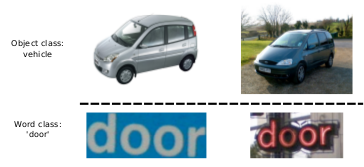
\includegraphics[scale=0.5]{img/object_recognition.png} }
		\caption[Reconocimiento generico de objetos]{Reconocimiento de palabras. Se considera a la palabra como una categoría de objeto al igual que la categoría ``vehiculo'' presentada en la parte superior de la imagen.}
		\label{fig: Reconocimiento generico}
	\end{figure}
